\documentclass[10pt,a4paper]{article}

\usepackage[utf8]{inputenc}
\usepackage[T1]{fontenc}
\usepackage{lmodern}
\usepackage[top=0.40in, bottom=0.40in, left=0.50in, right=0.50in]{geometry}
\usepackage{graphicx}
\usepackage{booktabs}
\usepackage{tabularx}
\usepackage{array}
\usepackage{amsmath,amssymb}
\usepackage{xcolor}
\usepackage{hyperref}
\usepackage{caption}
\usepackage{enumitem}
\usepackage{titlesec}
\usepackage{fancyhdr}
\usepackage{colortbl}
\usepackage{float}

% Academic Palette
\definecolor{NavyBlue}{RGB}{31, 78, 121}
\definecolor{TableHead}{RGB}{31, 78, 121}
\definecolor{HighlightRow}{RGB}{253, 237, 236}
\definecolor{AltRow}{RGB}{248, 249, 250}
\definecolor{TextDark}{RGB}{26, 26, 26}
\definecolor{MutedGray}{RGB}{102, 102, 102}

\hypersetup{
    colorlinks=true,
    linkcolor=NavyBlue,
    citecolor=NavyBlue,
    urlcolor=NavyBlue
}

% Section styling - standard black title, crisp academic navy section headers
\titleformat{\section}
  {\normalfont\normalsize\bfseries\color{NavyBlue}}{\thesection.}{0.4em}{}[\titlerule]
\titleformat{\subsection}
  {\normalfont\small\bfseries\color{NavyBlue}}{\thesubsection}{0.4em}{}

\titlespacing*{\section}{0pt}{4.5pt}{2pt}
\titlespacing*{\subsection}{0pt}{3pt}{1.5pt}

\setlist[itemize]{itemsep=1.5pt, topsep=1.5pt, partopsep=0pt, parsep=0pt, leftmargin=1.2em}
\setlist[enumerate]{itemsep=1.5pt, topsep=1.5pt, partopsep=0pt, parsep=0pt, leftmargin=1.2em}

\captionsetup{font=footnotesize, labelfont={bf,color=NavyBlue}, skip=2pt}

\pagestyle{fancy}
\fancyhf{}
\renewcommand{\headrulewidth}{0pt}
\fancyfoot[C]{\footnotesize \thepage\ of 3}

\setlength{\parindent}{0pt}
\setlength{\parskip}{2.8pt}

\setlength{\abovedisplayskip}{3.5pt}
\setlength{\belowdisplayskip}{3.5pt}

\begin{document}
\fontsize{9.5pt}{12.2pt}\selectfont

% =============================================================
% PAGE 1: HEADER, TITLE, AUTHORS, ABSTRACT, SEC 1, FIG 1, OBJECTIVES
% =============================================================
\noindent
\begin{minipage}[c]{0.12\textwidth}
    \centering
    
\includegraphics[height=2.0cm]{Docs/iut_logo.png}
\end{minipage}%
\begin{minipage}[c]{0.76\textwidth}
    \centering
    {\fontsize{11.5}{13.5}\selectfont \textbf{ISLAMIC UNIVERSITY OF TECHNOLOGY (IUT)}}\\[1pt]
    {\fontsize{8.5}{10.5}\selectfont \textbf{ORGANISATION OF ISLAMIC COOPERATION (OIC)}}\\[2pt]
    {\fontsize{10}{12}\selectfont \textbf{\color{NavyBlue}DEPARTMENT OF ELECTRICAL AND ELECTRONIC ENGINEERING}}\\[1pt]
    {\fontsize{8.5}{10}\selectfont \textit{B.Sc. Project and Thesis Synopsis (EEE 4700 / EEE 4800)}}
\end{minipage}%
\begin{minipage}[c]{0.12\textwidth}
    \centering
    
\includegraphics[height=2.0cm]{Docs/oic_logo.png}
\end{minipage}

\vspace{-3pt}
\noindent\textcolor{NavyBlue}{\rule{\textwidth}{0.8pt}}
\vspace{1pt}

% Title - Standard Academic Black
\begin{center}
    {\fontsize{12.5}{15}\selectfont \textbf{Conformalized Discrete-Time Hazard Modeling for Multi-Horizon\\Handover Forecasting in Cellular Networks}}
\end{center}

\vspace{-3pt}
\noindent
\begin{tabularx}{\textwidth}{@{}X r@{}}
    \textbf{\color{NavyBlue}Submitted by Candidates:} & \textbf{\color{NavyBlue}Under the Supervision of:} \\
    \textbullet\ \textbf{Saadman Sakib} \textcolor{MutedGray}{(Student ID: 210021110)} & \textbf{Dr. Mohammad Tawhid Kawser} \\
    \textbullet\ \textbf{Adhnan Kalim} \textcolor{MutedGray}{(Student ID: 210021308)} & Professor, Department of EEE \\
    \textbullet\ \textbf{Evan Ashfaque} \textcolor{MutedGray}{(Student ID: 210021335)} & Islamic University of Technology (IUT) \\
\end{tabularx}

\vspace{6pt}

% Abstract
\noindent\textbf{\color{NavyBlue}Abstract} --- \textit{Long-Term Evolution (LTE) networks manage mobility via 3GPP Event A3, a heuristic trigger that executes only after serving link deterioration. This thesis formulates an uncertainty-aware multi-horizon handover forecasting framework using continuous drive-test signalling. Across four campaigns in Dhaka and Gazipur (57 drives, 10,260 1~Hz samples, 938 RRC-confirmed handovers), a gradient-boosted hazard model predicts handovers 1~s ahead at AUROC 0.933 and AUPRC 0.784 (11.7$\times$ precision lift over a 6.7\% prevalence floor) with calibrated probabilities (ECE 0.024) and distribution-free conformal risk bounds ($\mathbb{E}[L] \le \alpha$). The system demonstrates robust generalisation on an unobserved highway holdout (AUROC 0.927). A 22-study benchmark confirms this is the first framework combining multi-horizon lead times, grouped evaluation, and finite-sample risk guarantees.}

% -------------------------------------------------------------
% 1. MOTIVATION & PROBLEM FORMULATION
% -------------------------------------------------------------
\section{Motivation and Problem Formulation}

In LTE networks, seamless mobility is governed by 3GPP Event~A3: a neighbour cell's RSRP must exceed the serving cell by an offset margin ($M_{\text{offset}}$) for a Time-to-Trigger (TTT) before the handset transmits a measurement report. This mechanism is \textbf{reactive by construction}---handover execution cannot begin until the link has already degraded (Figure~\ref{fig:a3_event}). Live commercial networks suffer severe operational penalties from this reactive delay:
\begin{itemize}
    \item \textbf{High Event Density \& Churn:} \textbf{938 handovers occurred in 2.9 hours} (one every 11 s; median separation 3.5 s).
    \item \textbf{Ping-Pong Oscillation:} \textbf{24.5\% of all handovers} returned to the source cell within 15 s, wasting network capacity.
    \item \textbf{Radio Link Failures (RLF):} Links collapsed into RLF \textbf{341 times}, causing costly connection re-establishments.
    \item \textbf{Discarded Measurement Reports:} Of 7,385 dispatched A3 reports, \textbf{62.9\% were unacted upon} by the base station.
\end{itemize}

\begin{center}
    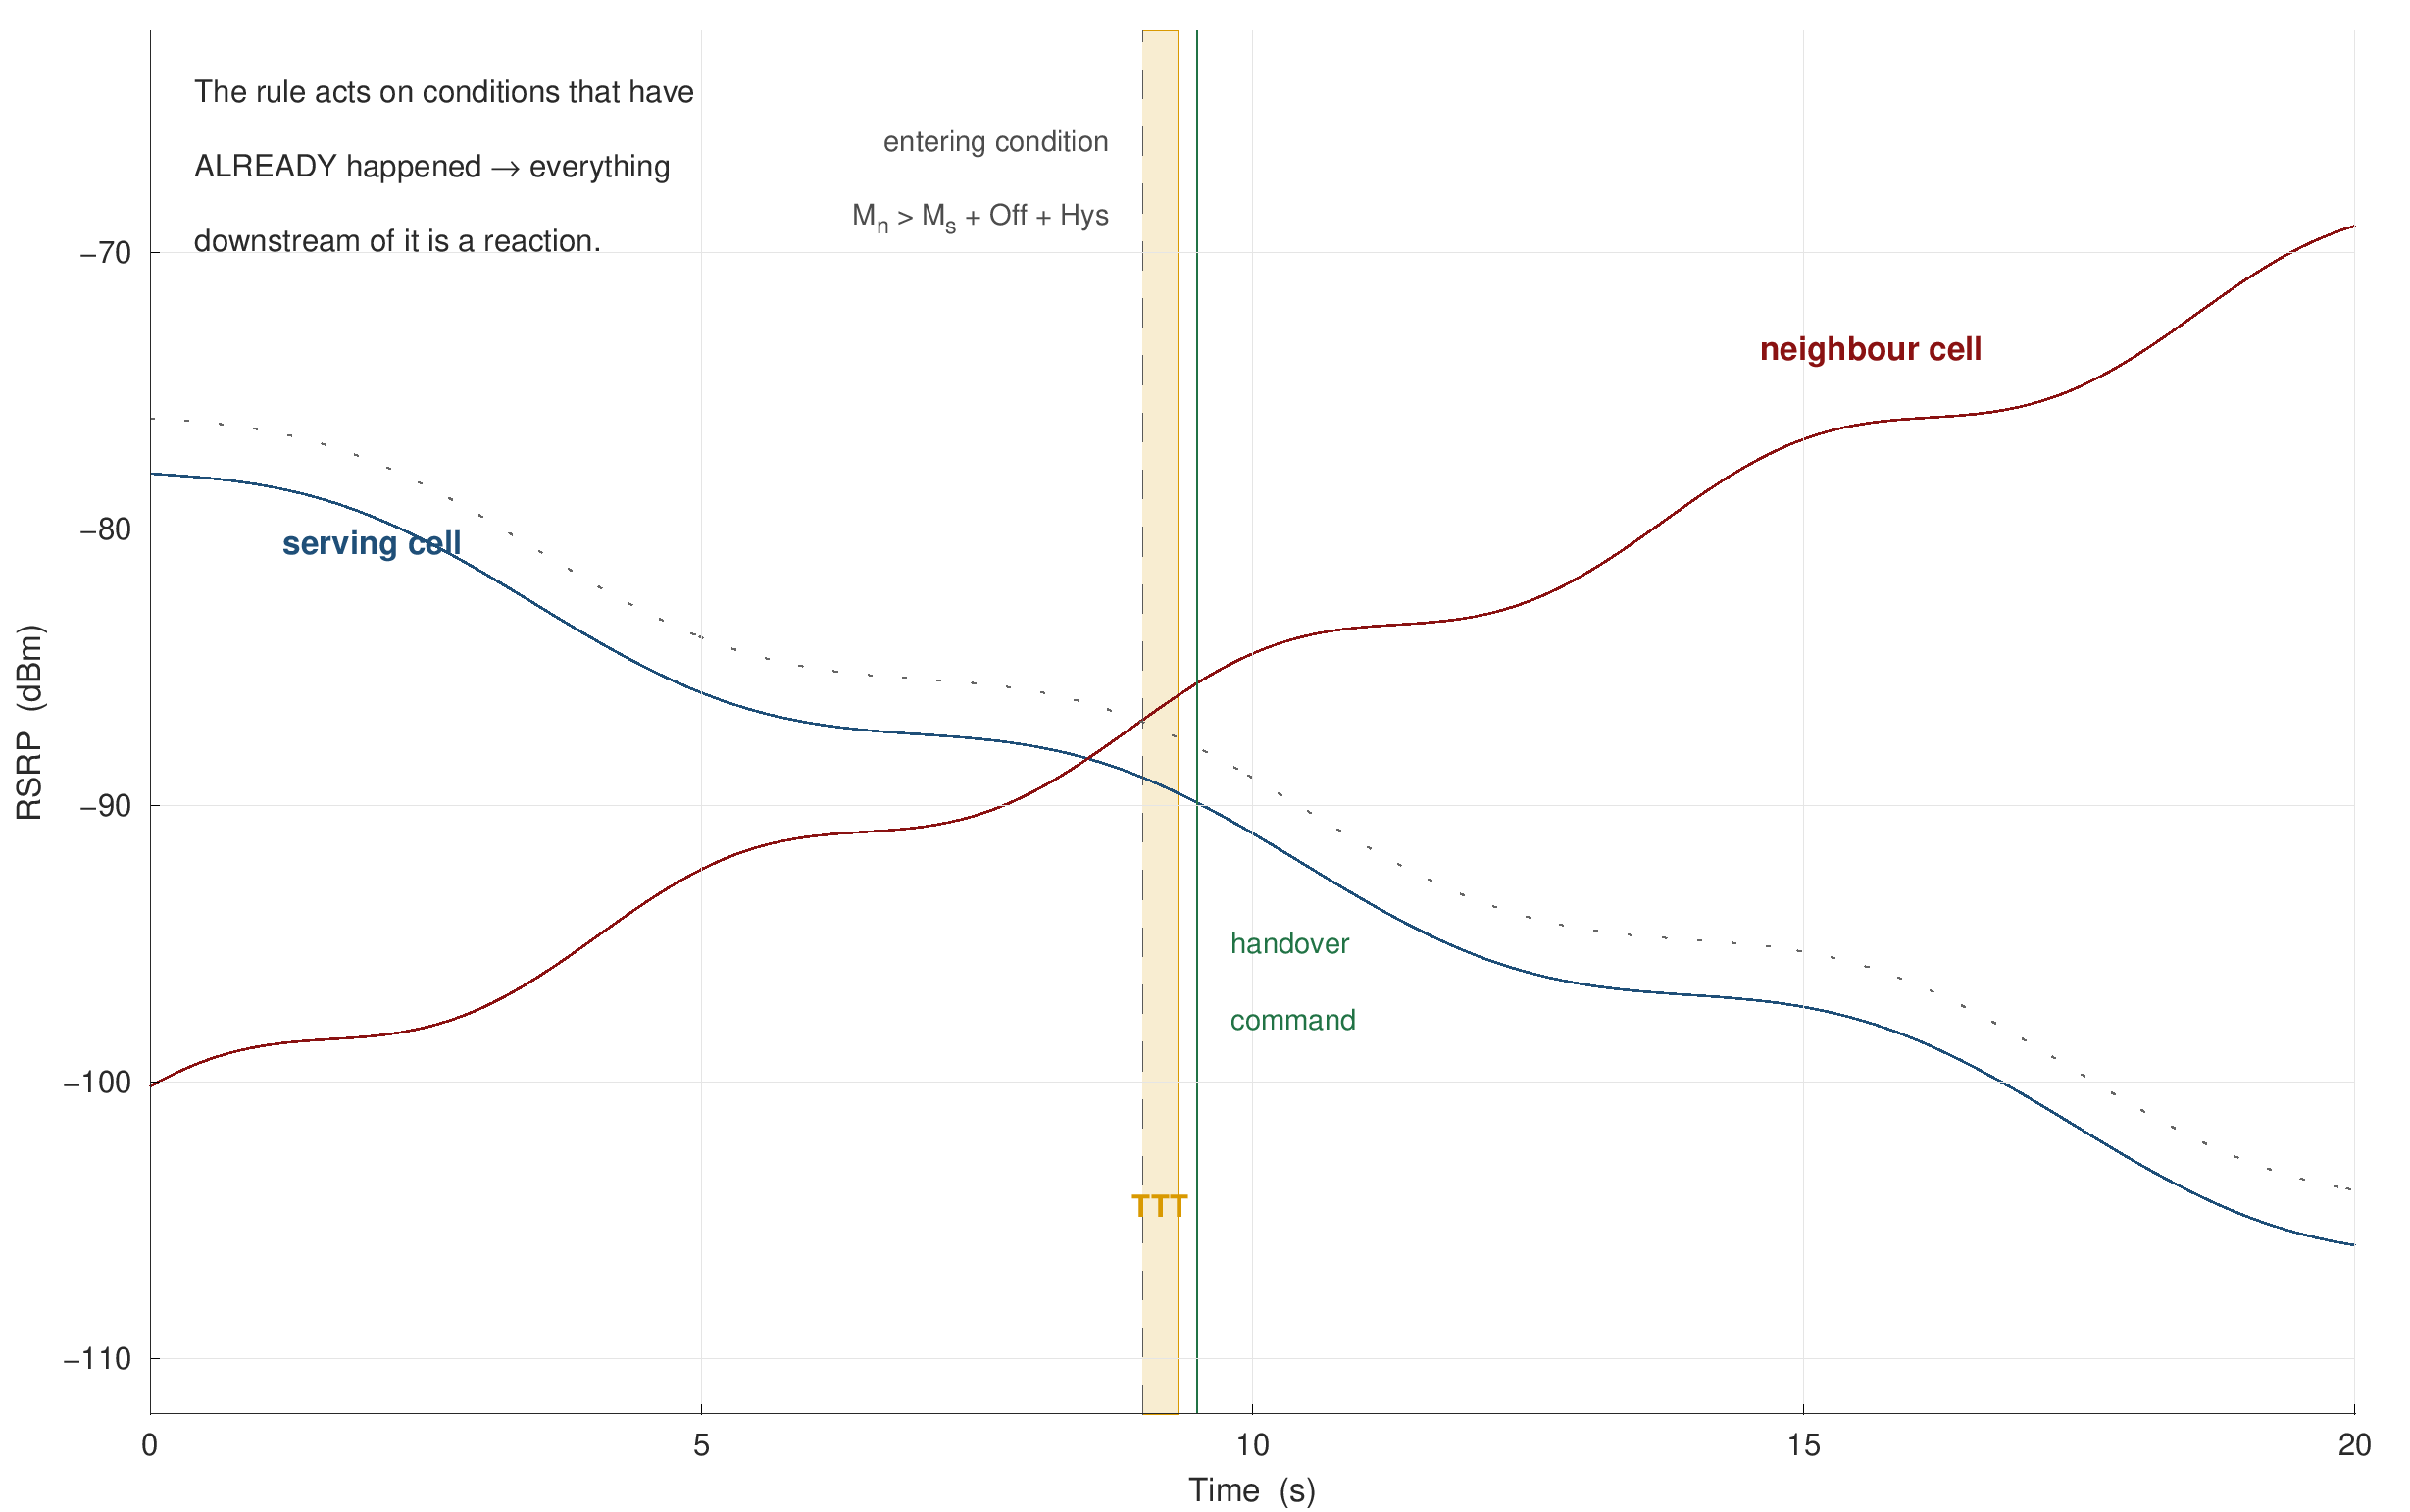
\includegraphics[height=5.8cm]{Presentation/figures/fig01_a3_event.png}
    \captionof{figure}{\textbf{Mechanics of 3GPP Event A3 Handover Trigger.} Handsets must wait for neighbour RSRP to exceed serving RSRP by $+1$~dB for a full 320~ms TTT before report dispatch, creating unavoidable reactive latency.}
    \label{fig:a3_event}
\end{center}

An audit of 22 published studies exposes three major scientific gaps: (1) no study enforces grouped whole-drive holdout evaluation, masking massive temporal leakage; (2) no model provides calibrated probabilities or finite-sample risk bounds; and (3) no prior work reports advance lead-time trade-offs.

\noindent\textbf{\color{NavyBlue}Formal Research Objectives:}
\begin{enumerate}
    \item[\textbf{O1:}] \textbf{Multi-Horizon Forecasting:} Forecast handovers across five discrete horizons ($h \in \{0.5, 1, 2, 3, 5\}$~s) using only UE signalling.
    \item[\textbf{O2:}] \textbf{Leakage-Free Benchmark:} Establish a grouped-drive clustered cross-validation protocol to eliminate temporal data leakage.
    \item[\textbf{O3:}] \textbf{Coherent Hazard Formulation:} Formulate a discrete-time hazard model guaranteeing 0.0\% horizon probability inversions.
    \item[\textbf{O4:}] \textbf{Unseen Highway Generalisation:} Validate domain transferability on an unobserved high-speed highway corridor (49.5 km/h).
    \item[\textbf{O5:}] \textbf{Mechanistic Network Dissection:} Dissect true operational handover parameters versus conventional static assumptions.
\end{enumerate}

\clearpage
% =============================================================
% PAGE 2: DATA & METHODOLOGY
% =============================================================
\section{Data Collection Methodology and Empirical Dataset}

\textbf{Drive-Test Measurement Infrastructure:} Field measurements were conducted using an engineering handset (Samsung Galaxy S10+, Samsung Exynos LTE-A baseband) running commercial \textbf{XCAL-M} diagnostics on Grameenphone LTE (Tier-1 operator, Bangladesh). XCAL recorded synchronous 1~Hz physical metrics (RSRP, RSRQ, RSSI, SINR, CQI across Bands 1, 3, and 8 with carrier aggregation) and decoded layer-3 RRC protocol packets (3GPP TS~36.331) capturing all reconfiguration, measurement, and re-establishment signalling.

\vspace{1pt}
\noindent
\begin{minipage}[c]{0.37\textwidth}
    \centering
    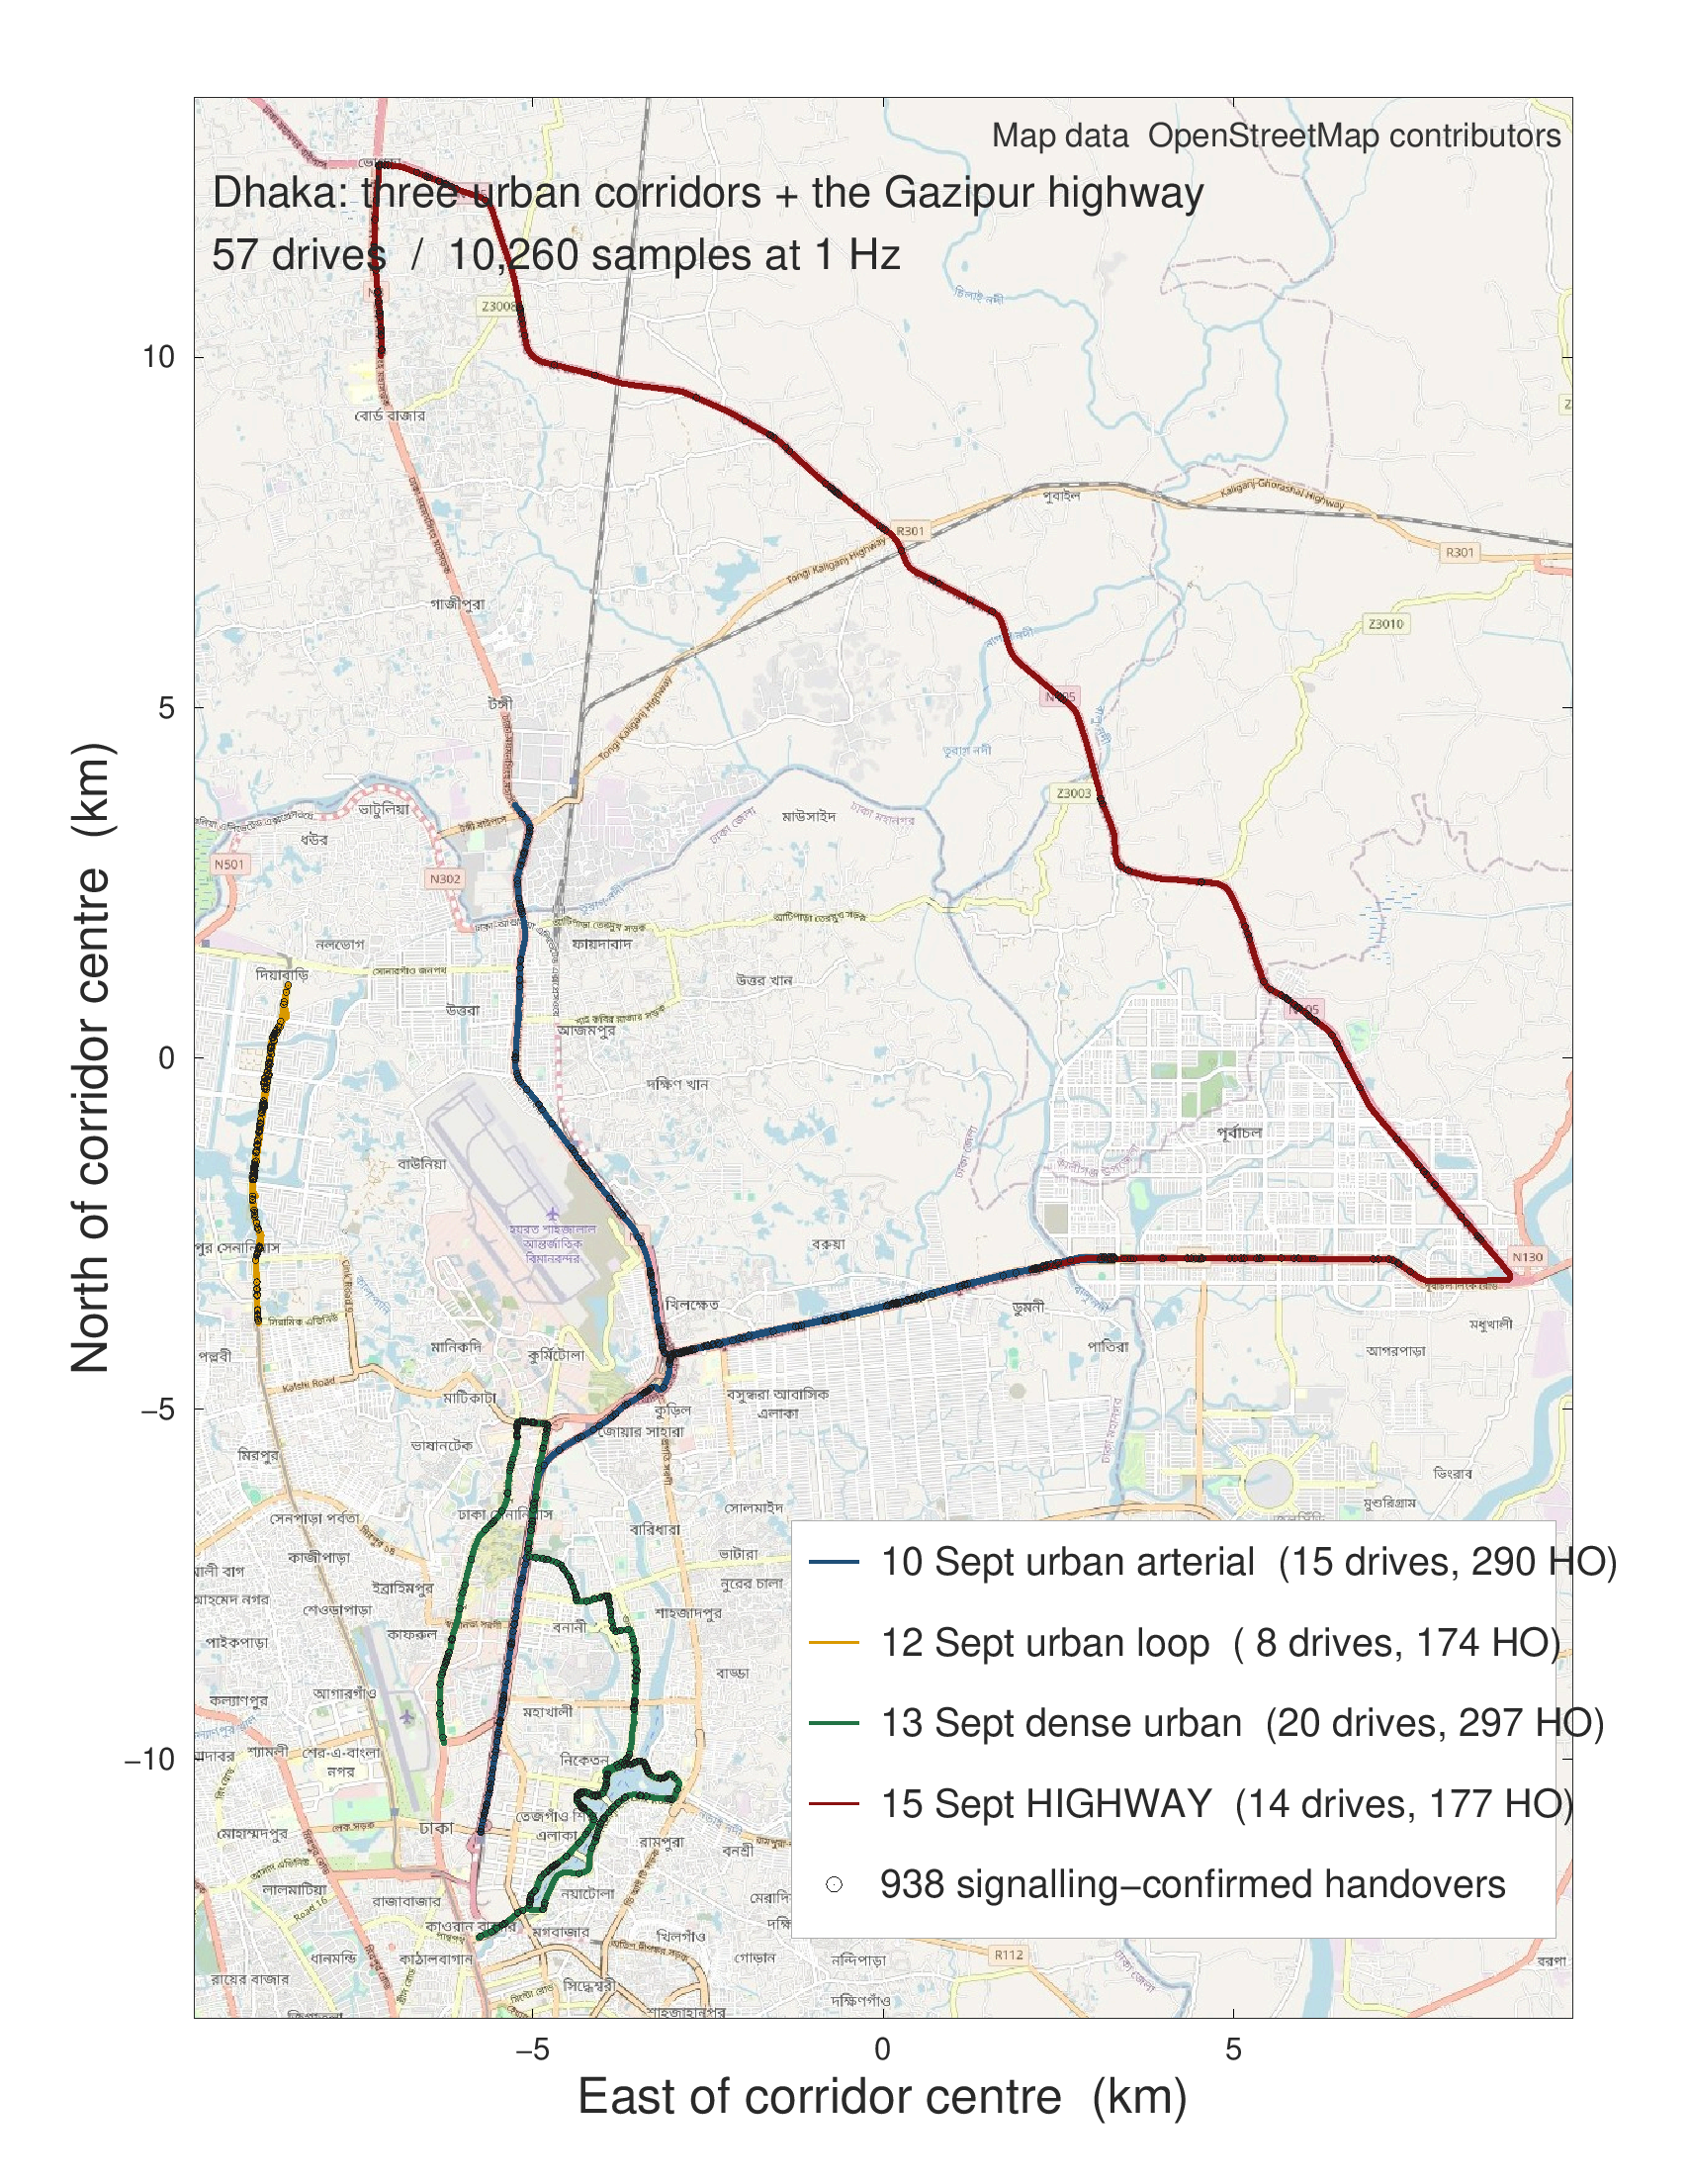
\includegraphics[height=7.2cm]{Presentation/figures/fig03_map_routes.png}
    \captionof{figure}{\textbf{Empirical Corridors across Dhaka and Gazipur.} 57 drives (938 handovers).}
    \label{fig:map_routes}
\end{minipage}\hfill
\begin{minipage}[c]{0.61\textwidth}
    \centering
    \captionof{table}{\textbf{Measurement Corpus Breakdown Across Campaigns}}
    \label{tab:dataset}
    \fontsize{7.8pt}{9.8pt}\selectfont
    \renewcommand{\arraystretch}{1.20}
    \begin{tabularx}{\linewidth}{@{}l l X c c c@{}}
    \toprule
    \rowcolor{TableHead}
    \color{white}\textbf{Campaign} & \color{white}\textbf{Region} & \color{white}\textbf{Corridor Regime} & \color{white}\textbf{Drives} & \color{white}\textbf{Samples} & \color{white}\textbf{HOs} \\
    \midrule
    1st Campaign & Tongi & Urban arterial & 15 & 2,700 & 290 \\
    \rowcolor{AltRow}
    2nd Campaign & Mirpur & Residential loop & 8 & 1,440 & 174 \\
    3rd Campaign & Dhaka Core & Commercial grid & 20 & 3,600 & 297 \\
    \rowcolor{AltRow}
    \textbf{4th Campaign} & \textbf{Gazipur} & \textbf{Highway (49.5 km/h)} & \textbf{14} & \textbf{2,520} & \textbf{177} \\
    \midrule
    \rowcolor{HighlightRow}
    \textbf{Pooled} & \textbf{Dhaka/Gazipur} & \textbf{Dual-regime corpus} & \textbf{57} & \textbf{10,260} & \textbf{938} \\
    \bottomrule
    \end{tabularx}
    \vspace{6pt}
    
    \fontsize{8.8pt}{11.4pt}\selectfont
    \textbf{Mobility Regimes:} (1) \textit{Urban Arterials \& Loops (1st--3rd Campaigns)}: dense microcell clutter, elevated metro-rail shadowing, stop-and-go congestion. (2) \textit{Highway Holdout (4th Campaign)}: logged on the Uttara--Gazipur expressway (peak speed $>70$~km/h) \textbf{after all models were frozen} for true out-of-distribution evaluation.
\end{minipage}

% -------------------------------------------------------------
% 3. METHODOLOGY & FORMULATION
% -------------------------------------------------------------
\section{Methodology and Mathematical Formulation}

\begin{center}
    \vspace{-1pt}
    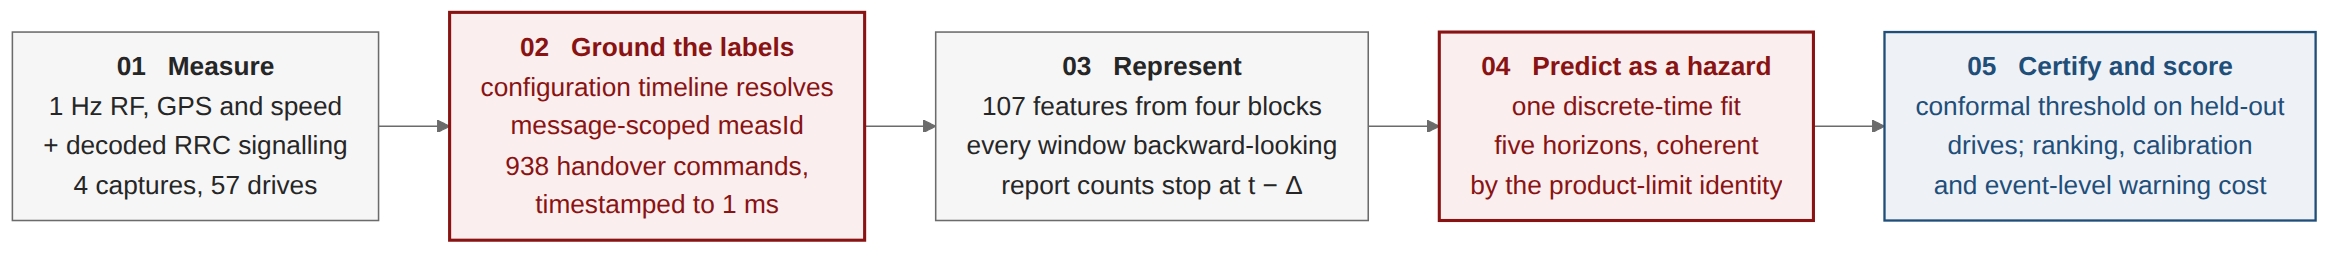
\includegraphics[width=\textwidth]{Presentation/figures/m14_framework.png}
    \vspace{-2pt}
    \captionof{figure}{\textbf{End-to-End System Architecture.} Stage~02 decodes RRC ground truth; Stage~03 extracts 107 clean features; Stage~04 fits discrete hazard survival model; Stage~05 certifies finite-sample distribution-free conformal risk bounds.}
    \label{fig:framework}
\end{center}

\textbf{Ground-Truth Signalling Replay:} Cell identity (PCI) changes in drive-test logs misdetect 42\% to 56\% of handovers due to averaging. We decode ground truth directly from \texttt{RRCConnectionReconfiguration} packets containing \texttt{mobilityControlInfo}. A stateful configuration timeline engine replays active \texttt{measId} and \texttt{reportConfigId} structures to track true network-triggered mobility.

\textbf{Horizon-Coherent Discrete-Time Hazard Formulation:} Independent binary classifiers across horizons $h \in \{0.5, 1, 2, 3, 5\}$~s cause \textbf{43.6\% horizon inversions} ($P(\text{HO} \le 1\,\text{s}) > P(\text{HO} \le 3\,\text{s})$). We formulate prediction as discrete-time survival analysis. Let $T$ denote the time to next handover. A single model estimates conditional per-second hazard $\lambda(t) = P(T = t \mid T \ge t, X_t)$:
\begin{equation}
P(T \le h \mid X_t) = 1 - \prod_{k=0}^{h-1} \bigl(1 - \lambda(t + k)\bigr) \quad \implies \quad \textbf{0.0\% inversions guaranteed by construction.}
\end{equation}

\begin{center}
    \vspace{-2pt}
    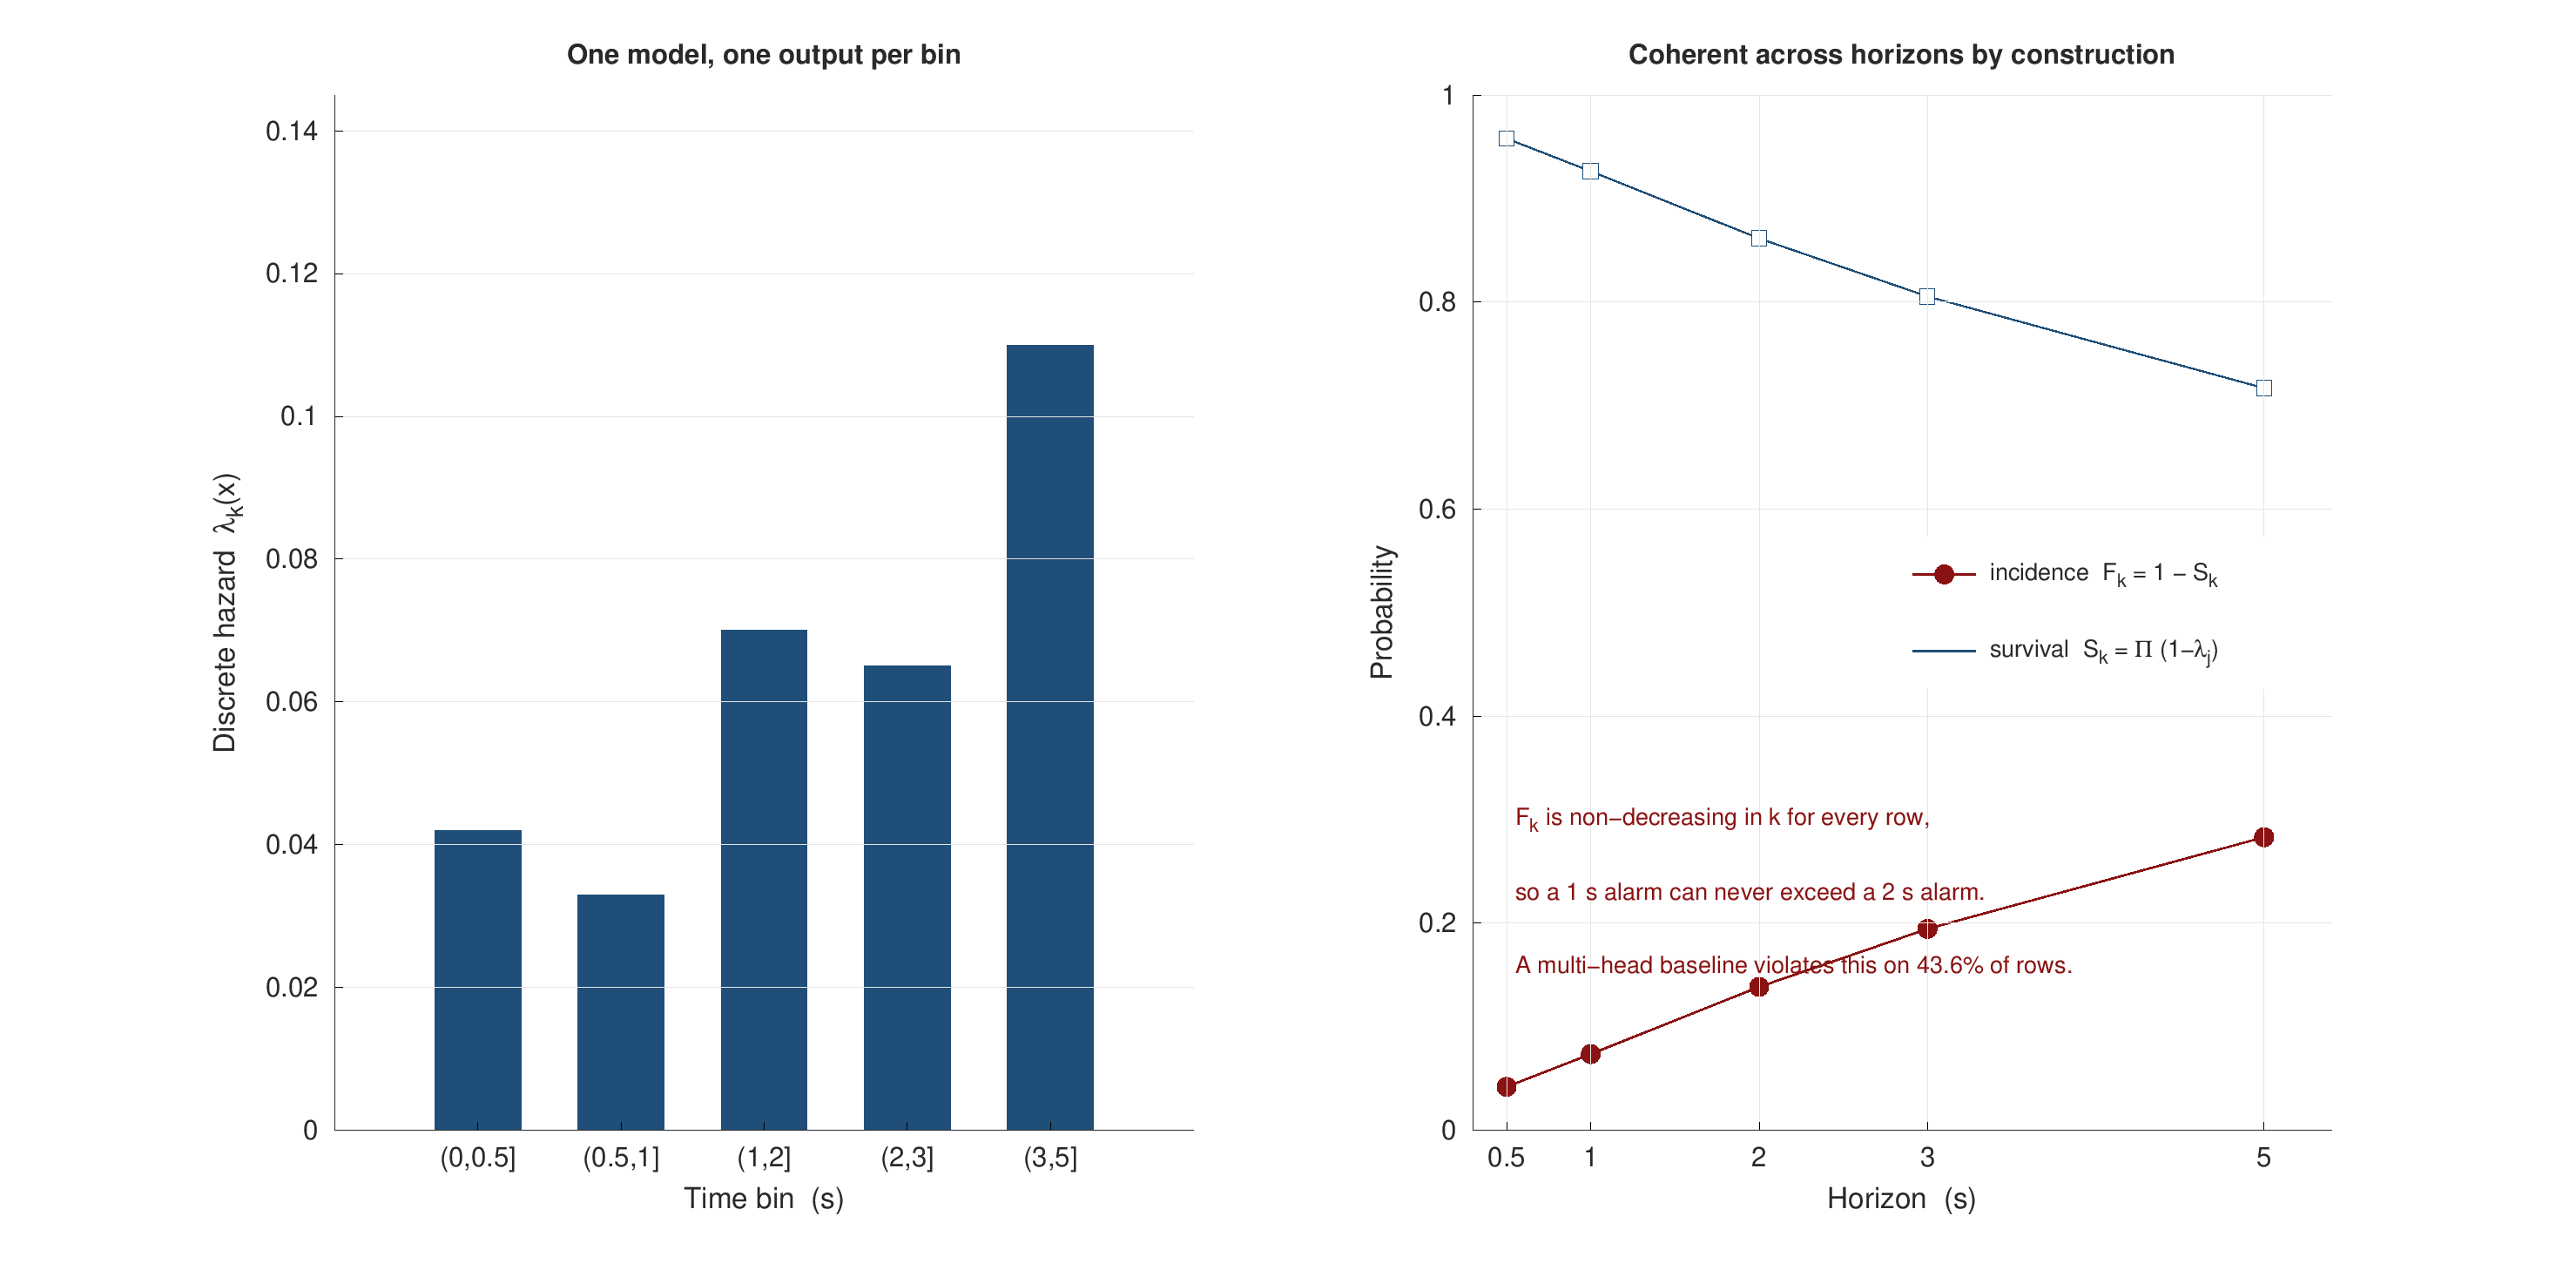
\includegraphics[height=3.4cm]{Presentation/figures/fig08_hazard_concept.png}
    \vspace{-3pt}
    \captionof{figure}{\textbf{Discrete-Time Hazard Formulation.} Left: Conditional hazard $\lambda_k(x)$ per time bin. Right: Monotonic cumulative incidence $P(T \le h \mid X)$ eliminating horizon inversions ($0.0\%$ vs $43.6\%$ in multi-head baselines).}
    \label{fig:hazard_concept}
\end{center}

\textbf{Feature Engineering and Clustered Protocol:} 107 leakage-free features survived multi-collinearity pruning across 4 blocks: 83 multi-window radio features (3/5/10~s stats, deltas, margins), 17 kinematic GPS features, and 7 dwell metrics. Folds are grouped by \textbf{whole drive} over a 4-fold rotation with 5 seeds (20 paired runs) and drive-level bootstrap confidence intervals.

\textbf{Conformal Risk Guarantees:} Decision thresholds are certified on 28 held-out calibration drives via Conformal Risk Control (CRC). For an operator loss tolerance $\alpha \in (0, 1)$, CRC guarantees that the expected per-drive miss rate satisfies:
\begin{equation}
\mathbb{E}[L_{\text{drive}}] \le \alpha \quad \text{with finite-sample, distribution-free statistical validity.}
\end{equation}

\clearpage
% =============================================================
% PAGE 3: RESULTS & BENCHMARK
% =============================================================
\section{Experimental Results and Literature Benchmark}

\noindent
\begin{minipage}[t]{0.49\textwidth}
    \centering
    \captionof{table}{\textbf{LightGBM Out-of-Fold Performance}}
    \label{tab:main_results}
    \fontsize{8.0pt}{10.0pt}\selectfont
    \renewcommand{\arraystretch}{1.22}
    \begin{tabularx}{\linewidth}{c c c c c}
    \toprule
    \rowcolor{TableHead}
    \color{white}\textbf{$h$} & \color{white}\textbf{Prevalence} & \color{white}\textbf{AUPRC} & \color{white}\textbf{Lift} & \color{white}\textbf{AUROC} \\
    \midrule
    0.5 s & 0.037 (3.7\%) & 0.416 & 11.3$\times$ & 0.916 \\
    \rowcolor{HighlightRow}
    \textbf{1.0 s} & \textbf{0.067 (6.7\%)} & \textbf{0.784} & \textbf{11.7$\times$} & \textbf{0.933} \\
    2.0 s & 0.125 (12.5\%) & 0.627 & 5.0$\times$ & 0.854 \\
    \rowcolor{AltRow}
    3.0 s & 0.175 (17.5\%) & 0.598 & 3.4$\times$ & 0.816 \\
    5.0 s & 0.259 (25.9\%) & 0.606 & 2.3$\times$ & 0.783 \\
    \bottomrule
    \end{tabularx}
\end{minipage}\hfill
\begin{minipage}[t]{0.49\textwidth}
    \centering
    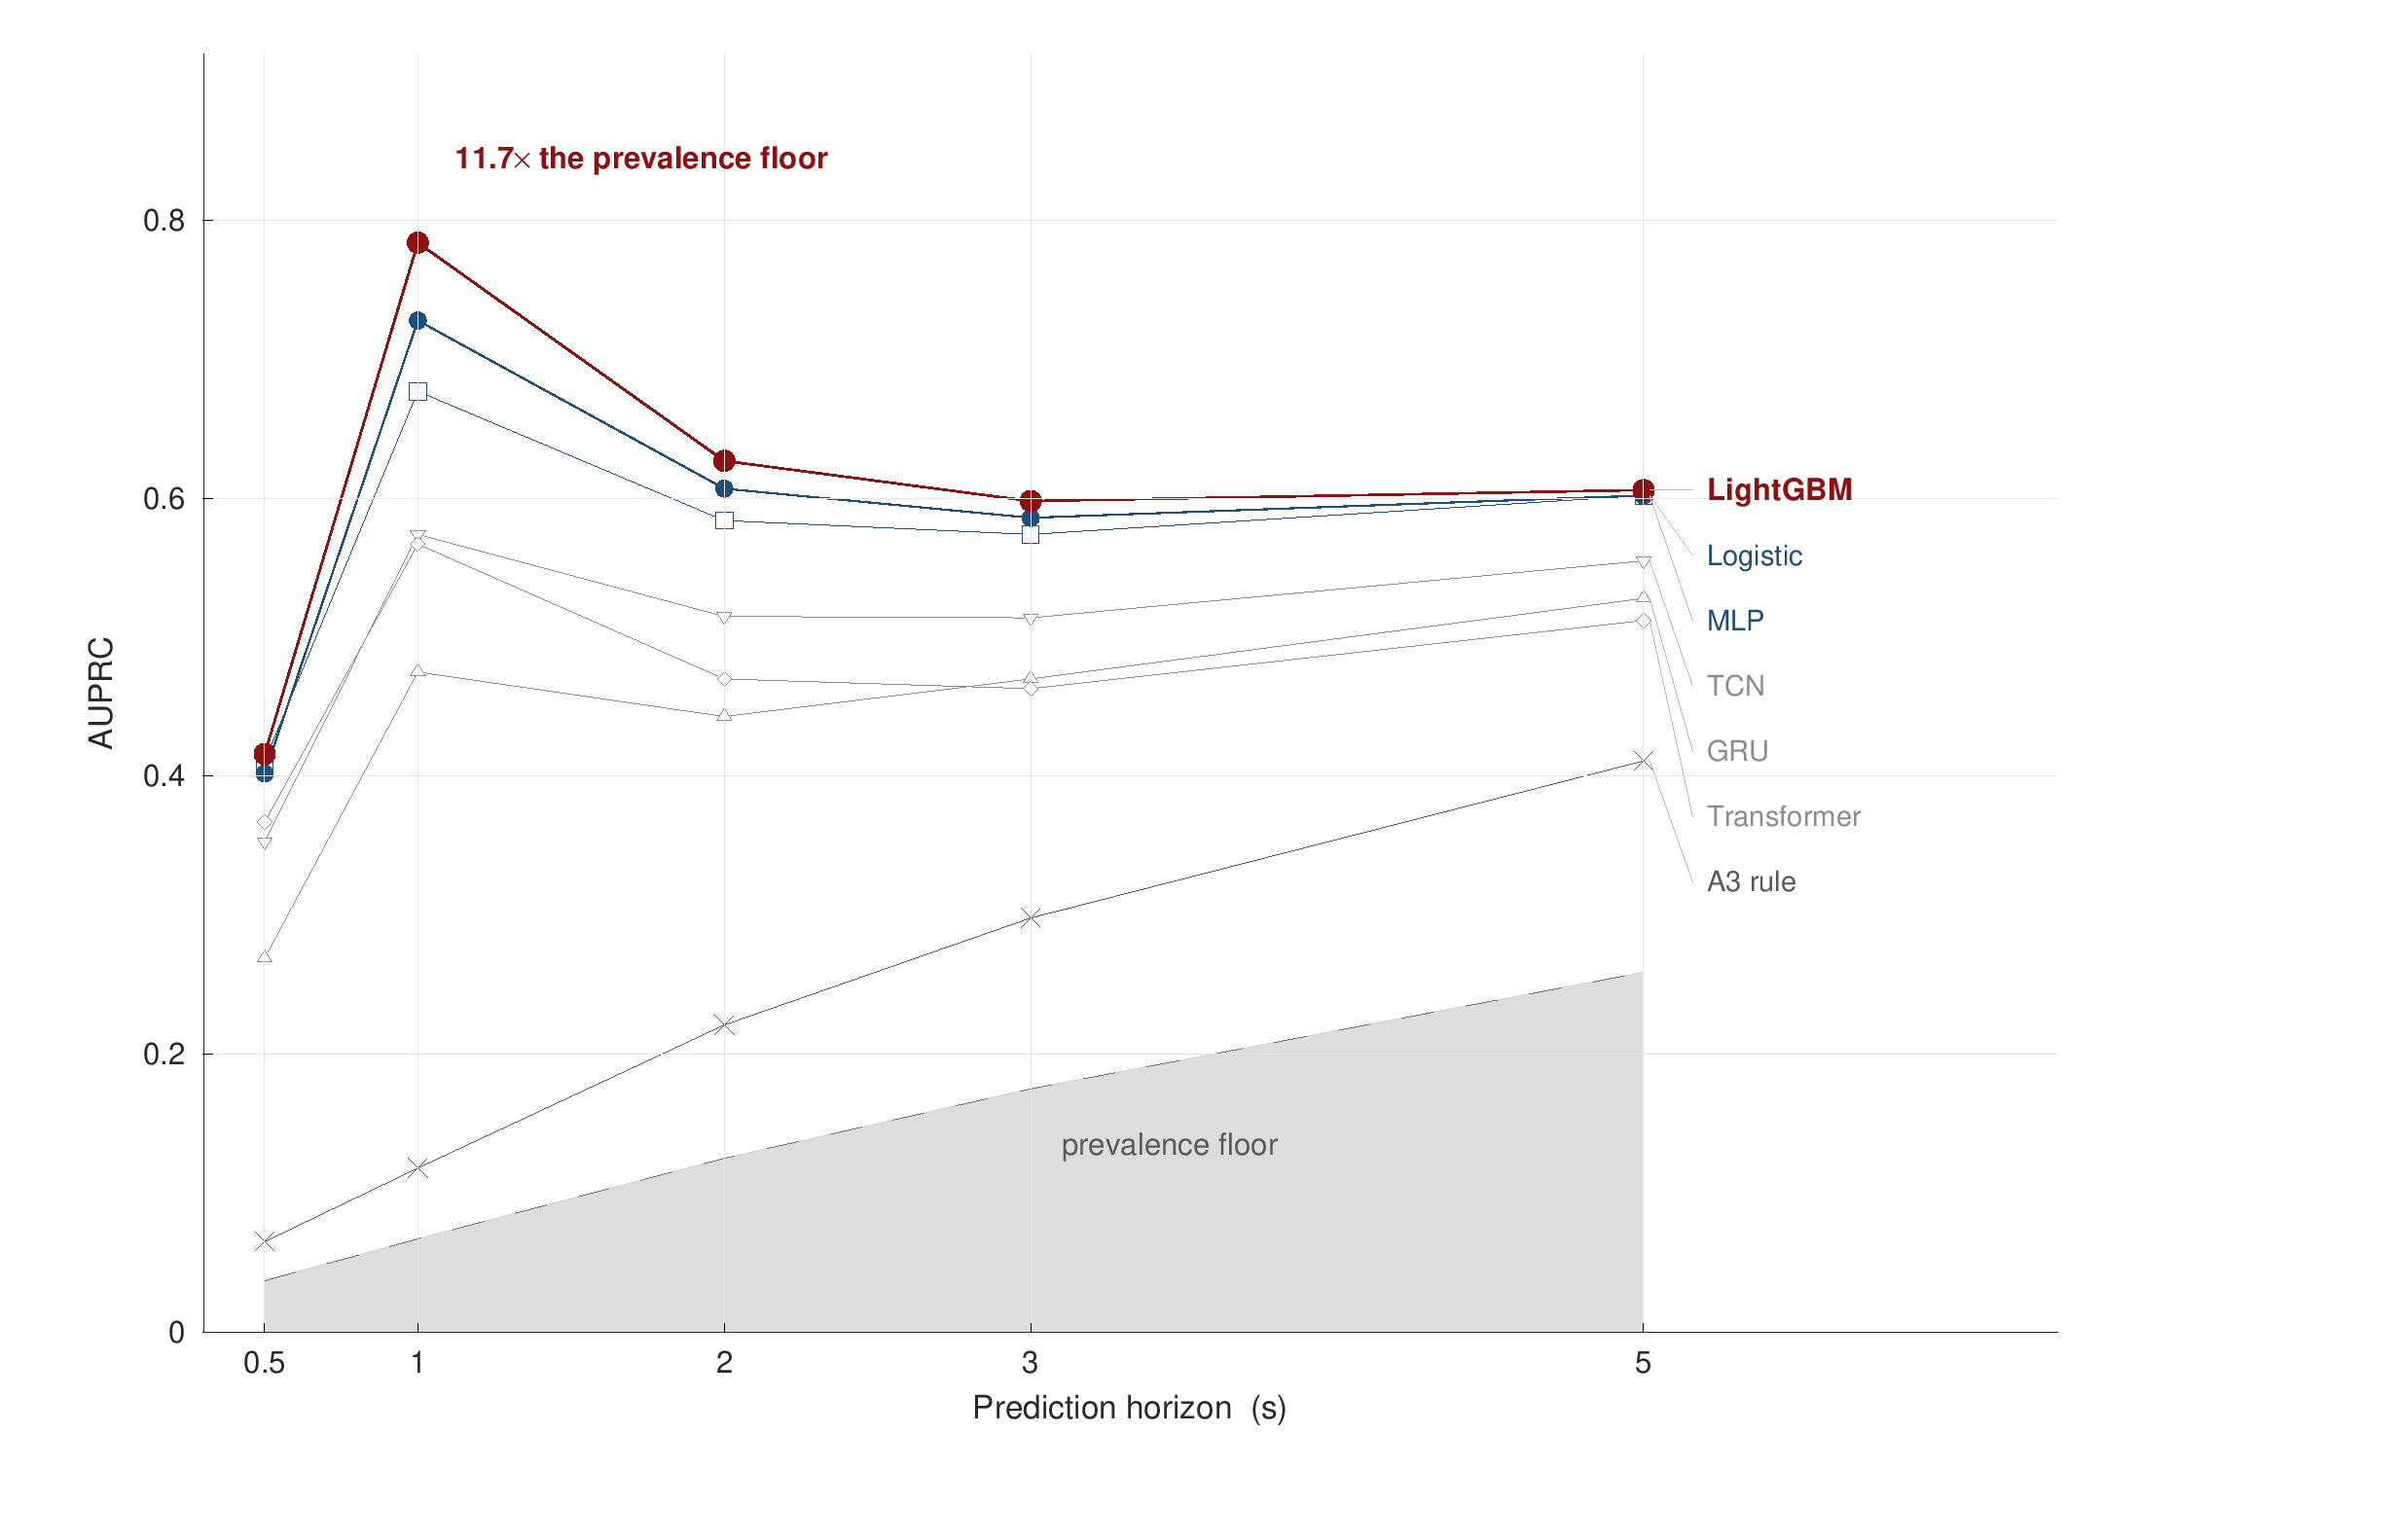
\includegraphics[height=5.6cm]{Presentation/figures/fig10_model_comparison.png}
    \captionof{figure}{\textbf{AUPRC vs. Horizon across Models.} LightGBM leads across all horizons (11.7$\times$ lift).}
    \label{fig:model_comp}
\end{minipage}

\vspace{3pt}
\captionof{table}{\textbf{Systematic Comparative Benchmark Across 22 Published Handover Prediction Studies}}
\label{tab:benchmark}
\fontsize{8.0pt}{10.2pt}\selectfont
\renewcommand{\arraystretch}{1.24}
\begin{tabularx}{\textwidth}{@{}p{3.5cm} X p{2.1cm} X X p{2.0cm}@{}}
\toprule
\rowcolor{TableHead}
\color{white}\textbf{Study \& Venue} & \color{white}\textbf{Data Source} & \color{white}\textbf{Split Protocol} & \color{white}\textbf{Primary Metric} & \color{white}\textbf{Calibration \& Risk} & \color{white}\textbf{Lead Time} \\
\midrule
\textbf{Boutiba et al. (2021)} [GLOBECOM] & 5G Testbed (OAI) & Unspecified (Leakage) & 98.03\% Accuracy (rare RLF) & None (Uncalibrated) & None (Fixed 5 steps) \\
\rowcolor{AltRow}
\textbf{Dzaferagic (2024)} [IEEE TNSM] & Real O-RAN (4,350 HOs) & Not Stated (Random row) & Precision / Recall (Single pt) & None (Uncalibrated) & None (Fixed horizon) \\
\textbf{Shafi et al. (2025)} [Mendeley/IUT] & Real XCAL Dhaka (2,154 pts) & Day 1 $\to$ Day 2 (n=1) & HO Count (AUROC 0.489) & None (Heuristic Q-table) & None (Reactive only) \\
\rowcolor{AltRow}
\textbf{Amirova et al. (2026)} [Future Int.] & Real LTE Astana (27k pts) & Device hold-out & PR curve, AUROC 0.82 & Bootstrap CI (No ECE) & None (Single horizon) \\
\midrule
\rowcolor{HighlightRow}
\textbf{This Work (2026) [IUT EEE]} & \textbf{Real LTE Dhaka (938 HOs)} & \textbf{Grouped whole-drive} & \textbf{AUPRC 0.416--0.784 (11.7$\times$)} & \textbf{ECE 0.024, CRC ($\ge$89\%)} & \textbf{0.5 s to 5.0 s (3.45s early)} \\
\bottomrule
\end{tabularx}

\vspace{3pt}
\textbf{\color{NavyBlue}Four Methodological Gaps Exposed in Literature:}
\begin{enumerate}[itemsep=3.0pt, topsep=2.5pt]
    \item \textbf{Fallacy of Raw Accuracy:} 7 of 22 papers report 94--99\% accuracy on imbalanced data. At 1~s (6.7\% prevalence), blindly predicting ``no handover'' scores \textbf{93.3\% accuracy} (and \textbf{96.3\%} at 0.5~s) while detecting zero true handovers. AUPRC and lift are mandatory.
    \item \textbf{Severe Temporal Data Leakage:} Random row splitting artificially inflates GRU AUPRC by \textbf{+74\% to +109\%} due to shadow-fading autocorrelation. Clustered whole-drive partitioning is strictly required.
    \item \textbf{Absence of Calibration:} Zero of 22 audited studies report probability calibration curves, ECE, or conformal risk bounds.
    \item \textbf{Departmental Head-to-Head (Shafi et al., 2025):} Under assumed static parameters ($M_{\text{offset}}=3$~dB, $\text{TTT}=1$~s), Shafi et al. yields AUROC 0.489. Our stateful RRC decode reveals 4 concurrent profiles with negative offsets ($-15$ to $+5$~dB), achieving AUROC \textbf{0.933} with \textbf{3.45~s advance warning}.
\end{enumerate}

% -------------------------------------------------------------
% 5. CONTRIBUTIONS
% -------------------------------------------------------------
\section{Summary of Key Contributions}
\begin{enumerate}[itemsep=3.0pt, topsep=2.5pt]
    \item \textbf{Discrete-Time Hazard Survival Formulation:} Eliminates probability inversions ($0.0\%$ vs $43.6\%$ in independent classifiers) from a single fit without ad-hoc post-processing.
    \item \textbf{Distribution-Free Conformal Risk Guarantees:} The first finite-sample exchangeable-drive risk control framework for cellular mobility, guaranteeing $\mathbb{E}[L_{\text{drive}}] \le \alpha$.
    \item \textbf{Quantification of Temporal Leakage Inflation:} Empirical proof that un-grouped data splitting inflates model metrics by $+4\%$ to $+74\%$.
    \item \textbf{Ground-Truth Signalling Replay:} A stateful timeline parser resolving active message-scoped measurement configurations, proving operational offsets on Grameenphone LTE are negative ($-15$ to $+5$~dB).
    \item \textbf{Empirical Operational Discoveries:} First quantification of the 62.9\% A3 report discard rate and layer-specific ping-pong concentration (31.0\% intra-carrier vs 6.5\% inter-carrier).
\end{enumerate}

% -------------------------------------------------------------
% 6. LIMITATIONS & REFERENCES
% -------------------------------------------------------------
\section{Limitations, Future Directions, and Key References}
\textbf{Limitations \& Future Work:} Bounded by 57 drives across one operator over four campaigns with 1~Hz export resolution (capping instant event detection at 90.5\%). Future work includes fuzzy regression-discontinuity design at the A3 margin, real-time O-RAN Near-RT RIC (xApp) deployment, and open dataset release.

\vspace{3pt}
\fontsize{7.8pt}{10.0pt}\selectfont
\textbf{Key References:}
[1] 3GPP TS 36.331 RRC Rel.~16, 2020.
[2] A.~Amirova et al., \textit{Future Internet} 18(2), 2026.
[3] A.~N.~Angelopoulos et al., \textit{ICLR}, 2024.
[4] K.~Boutiba et al., \textit{IEEE GLOBECOM}, 2021.
[5] A.~Cohen et al., \textit{IEEE Trans. Commun.}, 2022.
[6] M.~Dzaferagic et al., \textit{IEEE TNSM}, 2024.
[7] G.~Ke et al., \textit{NeurIPS}, 2017.
[8] S.~S.~Shafi, T.~Istiaque, M.~S.~Sowad, M.~T.~Kawser, \textit{Mendeley Data}, 2025.
[9] S.~Wiegrebe et al., \textit{Artif. Intell. Rev.} 57, 2024.
[10] A.~Zidic et al., \textit{Comput. Netw.} 227, 2023.

\end{document}
